\documentclass[preview]{standalone}

\usepackage{amsmath}
\usepackage{amssymb}
\usepackage{stellar}
\usepackage{definitions}
\usepackage{tikz}
\usepackage{wrapfig}
\usepackage{bettelini}

\usetikzlibrary{arrows.meta,positioning,decorations.markings,backgrounds,calc}

\tikzset{
    every node/.style={font=\footnotesize},
}

\begin{document}

\id{force-electromagnetic-fields}
\genpage

\section{Introduction}

\plain{The electromagnetic force is one of the four fundamental forces of nature.
It is responsible for the interactions between charged particles and is mediated by photons.}
\plain{The electromagnetic force can be described using electric and magnetic fields,
which are vector fields that exert forces on charged particles.
The electromagnetic force has a long range (in fact, it is infinite in range, just like gravity).}

\begin{snippetdefinition}{electric-field-definition}{Electric field }
    The \emph{electric field} \(\vec{E}(\vec{r})\) at a point \(\vec{r}\)
    in a space is defined as the electric force experienced by
    a unit positive charge placed at that point:
    \[
        \vec{E}(\vec{r}) = \frac{1}{4 \pi \epsilon_0} \frac{Q}{r^2} \hat{r}
    \]
\end{snippetdefinition}

\begin{snippetdefinition}{field-lines-definition}{Field lines}
    A \emph{field line} of a vector field \(\vec{F} \colon \realnumbers^n \to \realnumbers^n\) is a curve
    \(\vec{\gamma} \colon I \to \realnumbers^n\) such that its vector vector at each point
    is aligned with the vector field at that point:
    \[
        \frac{d\vec{\gamma}(t)}{dt} = \lambda(t) \vec{F}(\vec{\gamma}(t))
    \]
    for some scalar function \(\lambda(t) \neq 0\).
\end{snippetdefinition}

\begin{snippet}{field-liens-properties}
    The field lines: 
    \begin{itemize}
        \item are tangent to the vector field at each point;
        \item never intersect (if they did, the vector field would be undefined at that point);
        \item are denser where the field is stronger;
        \item for a single positive charge, they radiate outwards;
        \item for a single negative charge, they converge inwards;
        \item for a dipole, they emerge from the positive charge and terminate at the negative charge.
    \end{itemize}
\end{snippet}

\plain{Here are the field lines for a dipole:}

\includesnpt{dipole-field-lines-illustration}

\begin{snippetproposition}{field-lines-perpendicular-plane}{Field lines and equipotential surfaces}
    The field lines are perpendicular to a uniformly charged infinite plane.
\end{snippetproposition}

\begin{snippetproof}{field-lines-perpendicular-plane-proof}{field-lines-perpendicular-plane}{Field lines and equipotential surfaces}
    Consider a charge \(q\).
    Every particle on the plane exerts a force on \(q\).
    By symmetry, there is another particle 
    such that its force added to the first one
    has no component parallel to the plane.
    Thus, the total force on \(q\) has no component parallel to the plane.
    \begin{center}
    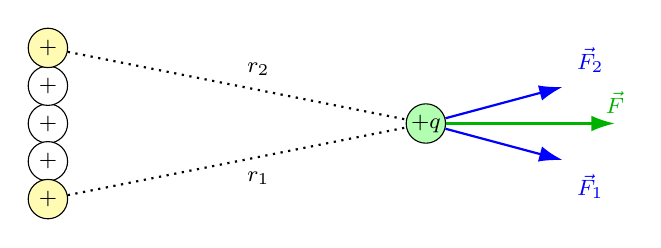
\begin{tikzpicture}[scale=1.2, 
        charge/.style={circle,draw,fill=white,minimum size=5mm,inner sep=0pt},
        force/.style={-{Latex[length=3mm,width=2mm]},thick},
        vec/.style={dotted,thick}
    ]

    % linea verticale di cariche positive
    \node[charge] (c0) at (0,0) {+};          % centrale
    \node[charge] (c1) at (0,0.4) {+};        % fra centrale e p1
    \node[charge,fill=yellow!30] (p1) at (0,0.8) {+}; % sopra evidenziata
    \node[charge] (c2) at (0,-0.4) {+};       % fra centrale e p2
    \node[charge,fill=yellow!30] (p2) at (0,-0.8) {+}; % sotto evidenziata

    % carica q a destra
    \node[charge,fill=green!30] (q) at (4,0) {$+q$};

    % raggi vettori verso q
    \draw[vec] (p1) -- (q) node[midway,above right] {$r_2$};
    \draw[vec] (p2) -- (q) node[midway,below right] {$r_1$};

    % forze su q (allineate alle linee, verso destra)
    \draw[force,blue] (q) -- ++(15:1.5) node[above right=2pt] {$\vec{F}_2$};
    \draw[force,blue] (q) -- ++(-15:1.5) node[below right=2pt] {$\vec{F}_1$};

    % risultante orizzontale
    \draw[force,green!70!black,thick] (q) -- ++(2,0) node[above] {$\vec{F}$};
    \end{tikzpicture}
    \end{center}
\end{snippetproof}

\begin{snippetproposition}{velocity-of-particle-in-uniform-field}{Velocity of a particle in a uniform electric field}
    Consider a particle of mass \(m\) with initial velocity \(\vec{v}_0\) in a uniform electric field \(\vec{E}\).
    After having traveled a distance \(s\) along the field lines,
    its velocity will be
    \[
        \vec{v} = \sqrt{v_0^2 + \frac{2Fs}{m}}
    \]
\end{snippetproposition}

\begin{snippetproof}{velocity-of-particle-in-uniform-field-proof}{velocity-of-particle-in-uniform-field}{Velocity of a particle in a uniform electric field}
    By the work-energy theorem,
    \[
        W = \Delta K = \frac{1}{2} m v^2 - \frac{1}{2} m v_0^2
    \]
    but this is equal to \(Fs\). By plugging this in we get
    \begin{align*}
        v^2 = v_0^2 + \frac{2Fs}{m}
    \end{align*}
\end{snippetproof}

\section{Quantization of charge (Millikan)}

\begin{snippet}{millikan-experiment-expl}
    \setlength{\intextsep}{0pt}%
    \begin{wrapfigure}{r}{8cm}
        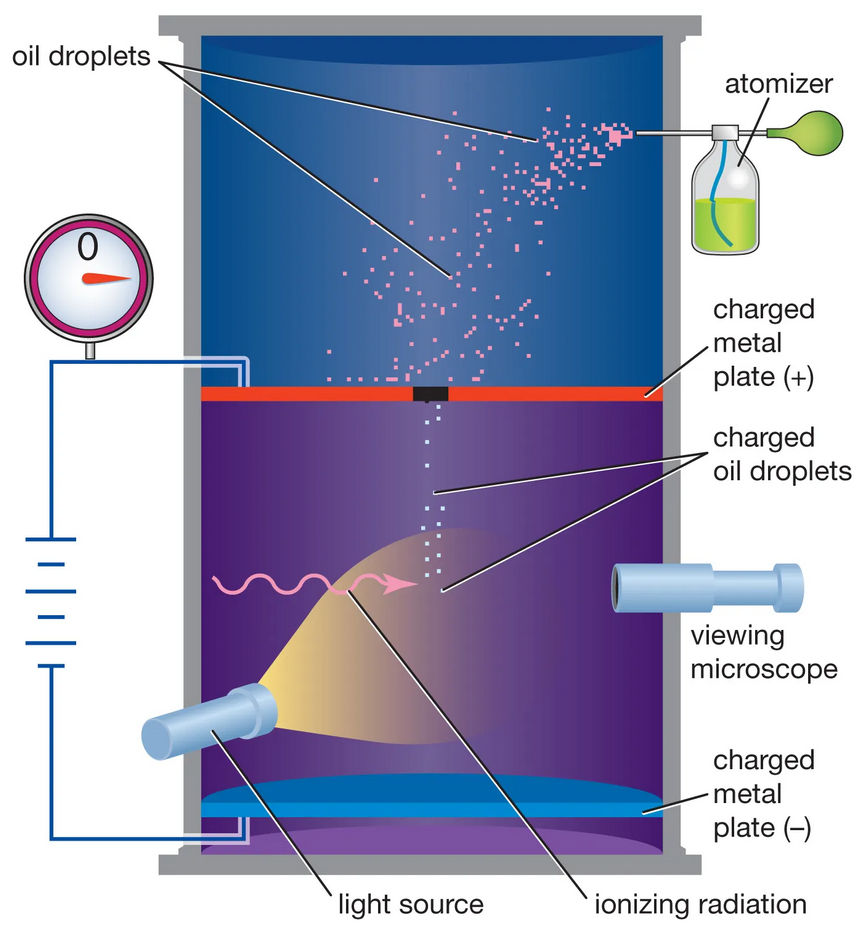
\includegraphics[width=7.5cm]{./resources/millikan.png}
        \vspace{-0.5cm}
    \end{wrapfigure}
    In 1909, Robert Millikan conducted his famous oil drop experiment to measure the charge of the electron \(e\).
    The setup consisted of:
    \begin{itemize}
        \item A fine mist of tiny oil droplets sprayed into a chamber.
        \item A vertical electric field applied between two parallel metal plates (made using two charged surfaces and a voltage source).
        \item A microscope to observe the droplets illuminated by a light beam.
    \end{itemize}
    The oil drops could become electrically charged by friction during spraying or by ionization from an external radiation source (like X-rays). Once charged, they were influenced by both gravity and the electric field.
    \wrapfill
    The forces acting on a droplet were:
    \begin{itemize}
        \item Gravitational force \(F_g = mg\) acting downward. Since the drop is spherical
        of radius \(r\) and density \(\rho\), its mass is \(m = \frac{4}{3} \pi r^3 \rho\).
        \item The viscous drag force \(F_d = 6 \pi \eta r v\) acting opposite to the direction of motion,
        where \(\eta\) is the viscosity of air and \(v\) is the velocity of the droplet (from Stokes' law).
        \item The electric force \(F_e = qE\) acting upward or downward depending on the charge \(q\) of the droplet and the direction of the electric field \(E\).
        \item The buoyant force \(F_b = \frac{4}{3} \pi r^3 \rho_{air} g\) acting upward, where \(\rho_{air}\) is the density of air.
    \end{itemize}
    When the electric field is off, the droplet eventually falls at its terminal velocity \(v_f\),
    where the drag balances gravity:
    \begin{align*}
        6\pi \eta r v_f &= \frac{4}{3} \pi r^3 (\rho- \rho_{air}) g \\
        r &= \sqrt{\frac{9\eta v_f}{2g(\rho - \rho_{air})}}
    \end{align*}
    When the electric field is applied and adjusted so the droplet is suspended (at rest), the electric force balances the effective weight:
    \begin{align*}
        qE &= \frac{4}{3} \pi r^3 (\rho - \rho_{air}) g \\
        q &= \frac{\frac{4}{3} \pi r^3 (\rho - \rho_{air}) g}{E}
    \end{align*}
    Repeating the experiment with many drops gave values of \(q\)
    that were always integer multiples of a smallest unit
    \[
        e \approx 1.602 \times 10^{-19} \text{ C}
    \]
\end{snippet}

\end{document}